\chapter{Conception et implémentation}



\section{Introduction}

L’outil d’aide à la décision pour le classement des salariés utilise les données issues de l’application de gestion du personnel d’une entreprise afin de faire un classement de ces derniers et en déduire les employés les plus méritants d’une promotion ou prime.\\
L’outil d’aide à la décision pour le classement des salariés utilise les données issues de l’application de gestion du personnel d’une entreprise afin de faire un classement de ces derniers et en déduire les employés les plus méritants d’une promotion ou prime.\\ 

\section{Architecture éventuelle de l’application }
L’application contiendra trois onglets principaux correspondant à trois modules différents :
\begin{enumerate}
\item L’onglet gestion du temps et absence
\item L’onglet gestion de l’activité quotidienne 
\item L’onglet informations personnelles 
\end{enumerate}

\subsection{Onglet gestion du temps et absence }

Cet onglet devrait contenir toutes les informations relatives aux absences (le nombre de jours où il s’est absent, les congés payés, les congés sans solde, les ponts, les RTT, ...etc).\\

Ces informations seront insérées par le salarié avant la fin du mois et validées par son manager à la fin du mois.

\subsection{Onglet gestion de l’activité quotidienne}

Dans cette section on retrouvera les informations relatives à l’activité quotidienne du salarié c’est-à-dire les taches qui lui sont affectées, la durée estimée pour leur réalisation, la durée réellement réalisée, la difficulté de la tâche, l’évaluation du travail effectué.\\
Le chef de projet s’occupe d’affecter les taches et d’estimer la durée de leur réalisation ainsi que leur difficulté en présence du n+1 du salarié et le salarié lui-même et cela durant les différentes réunions hebdomadaires par exemple.\\
Une fois la tache effectuée, le salarié insérera la durée réelle passée sur la tâche et qui pourrait s'avérer supérieure, égale ou inférieure à la durée estimée pour cette dernière.\\
Quant à l’évaluation du travail effectué, ça sera fait par le manager ou le n+1 et par le client (s’il y en a un) et cela en présence du salarié.          

\subsection{Onglet informations personnelles}

Cet onglet concerne plus les informations relatives au salarié telles que l'identifiant du salarié, nom, prénom, âge, adresse, numéro de téléphone, … le nombre d’années au sein de l’entreprise, le rang hiérarchique, les promotions et primes obtenues avec la date de chacune, le nombre total de promotion et prime obtenues, classement obtenu à la dernière réunion d’attribution de prime ou de promotion, une note d’appréciation.\\


Le salarié ainsi que ses supérieurs auront un accès en lecture seule sur ces informations, qui en réalité seront affichées directement de la base de donnée par le système en place. \\
La note d’appréciation quant à elle est calculée chaque mois par le système en utilisant les votes anonymes des salariés de l’entreprise. Le système d’évaluation propose 5 types d’appréciation d’après le tableau suivant :    

\begin{figure}[!h]
\begin{center}
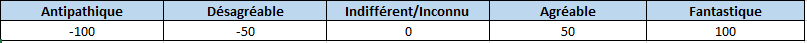
\includegraphics[height=0.8cm]{Conception_implementation/tableau_sym.png}
\end{center}
\caption{tableau notes salarié}
\end{figure}

En ce qui concerne le classement obtenu à la dernière réunion d’attribution de prime ou de promotion c’est justement le sujet principal de ce travail, j’en parlerai plus en détail dans les sections suivantes mais en générale le système calculs et retourne d’après différents critères appliqués aux salariés un classement de ces derniers du plus méritant d’une promotion (ou prime) au moins méritant, donc le classement obtenu lors de la dernière exécution du système sera affiché sur le profil du salarié .      

\section{Historisation Mensuelle}

A chaque fin de mois l’application fait une historisation des informations récoltées concernant chaque salarié de l’entreprise.  

\section{Analyse des données récoltées }

Afin de pouvoir faire un classement des salariés notre système a besoin d’un fichier Excel ou d’une Base de données directement en entrée.\\
Ce fichier Excel contiendra l’ensemble des actions, critères et poids dont le système a besoin pour effectuer le classement des salariés. Pour construire ce fichier, nous nous proposons d'utiliser l'ETL qui va effectuer une collecte de données à partir d’un magasin de données dédié à cet effet et récolter les mesures (indicateurs) qui nous intéressent sur les salariés et ce sous format Excel. \\
Le magasin de données sera construit toujours grâce à l’ETL durant la phase d’alimentation qui se fera à partir de la base de données de production. Et, c’est durant cette phase là que le calcul des indicateurs « mesures » se fera grâce aux requêtes analytiques.  \\
\newpage
Les indicateurs « mesures » choisi pour ce travail sont les suivants:
\begin{enumerate}
\item Les compétences et Les résultats (productivité de l’employé)   I1
\item Les appréciations sociales  I2
\item La pénibilité du travail   I3
\item L’ancienneté dans l'entreprise   I4
\item L’assiduité (Les présences et les absences)    I5
\end{enumerate}

\subsection{Compétences et Les résultats (productivité de l’employé)}
Cet indicateur est calculé à partir de l’évaluation du travail effectué et temps passé sur la tâche, et faire une moyenne des deux critères. \\
Le score obtenu pour l’évaluation du travail effectué est récupéré directement de la base de données et sa valeur est répartie entre 0 et 100. Quant au score obtenu pour le temps passé sur la tâche, il est déduit à partir de la règle suivante :\\

On part du principe que si un travail est effectué en temps voulu c’est-à-dire « durée estimée = durée réelle effectuée » alors le salarié obtient un score de 50\%. Et à partir de cette base là ,on calcule les autres scores, et pour exemple : un salarié ayant effectué une tache dont la durée était estimée à 5 jours en seulement  3 jours  aurait un score de 70\%.\\

Pour finir, on calculera la moyenne de ces scores sur tous les mois compris dans l’évaluation semestrielle ou annuelle.  La récupération de ces scores est possible grâce à l’historisation mensuelle.  


\subsection{Appréciations sociales}
Pour cet indicateur, on n'a pas besoin de calcul car on a déjà le score dans le format voulu grâce à l’application de vote anonyme dont les valeurs varient entre -100 et 100.   \\
Ensuite, on calculera la moyenne de ces scores sur tous les mois compris dans l’évaluation semestrielle ou annuelle, étant donné que le vote se fait de manière mensuelle. La récupération de ces informations est possible grâce à l’historisation mensuelle.

\subsection{Pénibilité du travail}
Comme pour l’indicateur précédent et comme expliqué plus haut, le score est déjà calculé et saisis par le chef de projet manuellement avec une notation entre 1 et 100.\\
Ensuite, on calculera la moyenne de ces scores sur tous les mois compris dans l’évaluation semestrielle ou annuelle et cela grâce à l’historisation mensuelle. 


\subsection{Ancienneté dans l'entreprise }
 Cet indicateur est calculé d’après le nombre d’années passées dans l’entreprise, à savoir directement le nombre d’années compris entre 0 et 40 ans.\\
Cet indicateur est mis à jour chaque année. 


\subsection{Assiduité « les présences et les absences »}
Le calcul de cet indicateur se fera mensuellement suivant le principe utilisé pour le calcul du premier indicateur « I1 », c’est-à-dire qu'on considère pour une personne qui a 0 absence durant le mois équivaut à 100\%, et à partir de cette règle, on en déduira les autres.\\
Ensuite, on calculera la moyenne de ces scores sur tous les mois compris dans l’évaluation semestrielle ou annuelle grâce à l’historisation mensuelle. 


\section{Classement des salariés }
L’outil d’aide à la décision pour le classement des salariés, Prend en entrée un fichier Excel « que je suppose déjà crée » contenant la matrice de performance et retourne un classement des salariés sur un autre fichier Excel.\\ 
Pour effectuer cela, j’ai choisis de tester deux méthode d’analyse multicritère LA SOMME PONDÉRÉE et ELECTRE III.\\

Le premier et deuxième point de ce qui suit concernent les démarches communes effectuées pour les deux méthodes

\begin{enumerate}
\item Détermination des critères :
\\
J’ai choisis 5 critères pertinents après avoir questionné quelques Managers.
      \begin{itemize}
      \item Les compétences et Les résultats (productivité de l’employé)
      \item Les appréciations sociales
      \item La pénibilité du travail
      \item L’ancienneté dans l'entreprise
      \item Les présences et les absences     
      \end{itemize}
      
\begin{figure}[!h]
\begin{center}
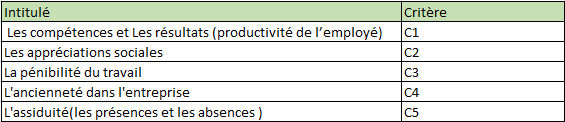
\includegraphics{Conception_implementation/noms_criteres.png}
\end{center}
\caption{Le tableau des critères retenus}
\end{figure}

\newpage

\item Pondération des critères :
\\
Le premier et deuxième point de ce qui suit concernent les démarches communes effectuées pour les deux méthodes

\begin{figure}[!h]
\begin{center}
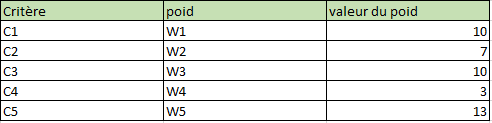
\includegraphics{Conception_implementation/poids.png}
\end{center}
\caption{Le tableau de pondération des critères 1}
\end{figure}


Le tableau des poids utilisé en entré du programme :
\begin{figure}[!h]
\begin{center}
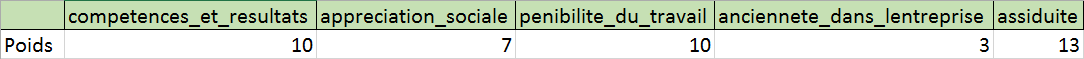
\includegraphics[width=16cm]{Conception_implementation/poids_en_entr_s.png}
\end{center}
\caption{Le tableau de pondération des critères 2}
\end{figure}


\item Détermination des seuils :
\\
J’ai choisi de donner la même valeur de seuil de préférence et de seuil d’indifférence a tous les critères Pj = Qj = 0 pour avoir le cas particulier de vrai critère et éviter le cas d’incomparabilité « aQb » et d’indifférence « aIb » entre deux action.

\begin{figure}[!h]
\begin{center}
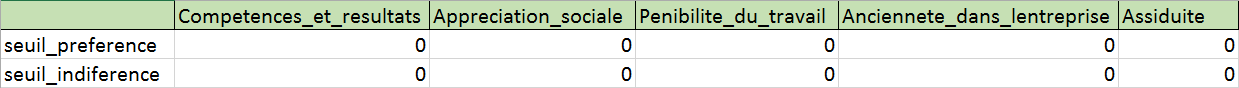
\includegraphics[width=16cm]{Conception_implementation/seuils.png}
\end{center}
\caption{Le tableau des seuils de préférences et d’indifférences attribués aux critères}
\end{figure}

Pour le veto, les valeurs sont différentes d’après l’importance du critère. Sur certains l’effet de veto est supprimé, considérant de façon arbitraire que la nature de ces critères n’amène pas forcément à refuser le sur-classement d’une action sur l’autre si la différence de leur performance dépasse une certaine valeur.    

\begin{figure}[!h]
\begin{center}
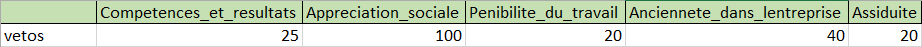
\includegraphics{Conception_implementation/veto.png}
\end{center}
\caption{Le tableau des seuils de préférences et d’indifférences attribués aux critères}
\end{figure}

\end{enumerate}

\newpage


\section{Implémentation}

 Pour effectuer le classement des salariés, on avait choisi de tester deux méthodes d’analyses multicritère à savoir la somme pondérée et ELECTRE III, que j’ai implémenté avec le langage python.


\subsection{ELECTRE }
\subsubsection{Évaluation des indices de concordance :}
La fonction qui permets de vérifier la concordance partielle :
\begin{lstlisting}[language=Python, frame=single, firstnumber=127]
def concord_parti(gs1, gs2, critere):
    if gs1 >= gs2 - seuil_indiference[critere]:  
        return 1
    elif gs1 <= gs2 - seuil_preference[critere]:  
        return 0
    else:
        return (seuil_preference[critere] - (gs2 - gs1)) / (seuil_preference[critere] - seuil_indiference[critere])
\end{lstlisting}

\subsubsection{Calcul de l’indice de la concordance globale :}
La fonction qui permets de calculer l’indice de la concordance globale :

\begin{lstlisting}[language=Python, frame=single, firstnumber=137]
def concord(s1, s2):
    conc = 0.0
    for critere in Criteres:
        poids = Poids[critere]
        
        gs1 = Performances[s1][critere]
        gs2 = Performances[s2][critere]
        c = concord_parti(gs1, gs2, critere)
        conc += c * poids
        
    print("    concordance entre : "+s1+" et "+s2+" est : "+str(conc) )
    return conc  
\end{lstlisting}

\subsubsection{Évaluation des indices de discordance partielle:}
\begin{lstlisting}[language=Python, frame=single, firstnumber=90]
def discord_parti(gs1, gs2, veto, critere):
    diff = gs2-gs1
    if (gs1 < 0) & (gs2 < 0) :
        diff = abs(gs2 - gs1)
        
    if diff >= veto:
        return 1
    elif diff <= seuil_preference[critere]:
        return 0
    else :
        res = 1 - ((veto - diff)/(veto - seuil_preference[critere]))
        return res
\end{lstlisting}

\newpage

\subsubsection{Évaluation des indices de discordance globale:}
\begin{lstlisting}[language=Python, frame=single, firstnumber=106]
def discord(s1, s2, conc):
    app_disc = appliquer_disc(s1, s2, conc)
    disc = 1.0
    if app_disc == True:
        for critere in Criteres:
            veto = vetos[critere]
            gs1 = Performances[s1][critere]
            gs2 = Performances[s2][critere]
            d = discord_parti(gs1, gs2, veto, critere)
            if d > conc :
                tmp = (1-d)/(1-conc)
                disc *=  tmp
                   
        print("        discordance entre : "+s1+" et "+s2+" est : "+str(disc) )
    return disc
\end{lstlisting}

\subsubsection{Calcul de l’indice de crédibilité :}
\begin{lstlisting}[language=Python, frame=single, firstnumber=157]
def credibilite(ks1, ks2):
    conc = concord(ks1, ks2)
    disc = discord(ks1, ks2, conc)
    cred = conc * disc
    return cred
\end{lstlisting}


\subsubsection{Le classement des salariés}
\begin{lstlisting}[language=Python, frame=single, firstnumber=157]
# retourne meilleur entre 2 salaries
def compare_2_salarie(ks1, vs1, ks2, vs2):
    print("Calcule credibilite entre "+ks1+" et "+ks2+" et l'inverse : ")
    cred1 = credibilite(ks1, ks2)
    cred2 = credibilite(ks2, ks1)
    print("credibilite "+ks1+" et "+ks2+" : "+str(cred1))
    print("credibilite "+ks2+" et "+ks1+" : "+str(cred2))
    if cred1 >= cred2:
        print("*********** "+ks1+" surclasse "+ks2+" *********** ")
        return ks1, vs1
    else :
        print("*********** "+ks2+" surclasse "+ks1+" *********** ")
        return ks2, vs2
\end{lstlisting}
\newpage
\subsection{Somme pondéré }
\subsubsection{Normalisation des données }
Cette fonction permet à partir de la matrice de décision (le tableau des performances) d’aboutir à une matrice normalisée, j’ai choisis la procédure de normalisation suivante  : \\
n étant le nombre de critères, on a:
\begin{align*}
v_{i} = \frac{a_{i}}{\sum_{i=1}^{n}a_{i} }, \forall i \in [1, m]
\end{align*}
\begin{lstlisting}[language=Python, frame=single, firstnumber=63]
def normalisation_data(performances):
    print("\n\n")
    print("************************ donnees normalisees ************************")
    for p in performances.keys():
        somme_ligne = sum(performances[p].values())
        for c in performances[p].keys():
            performances[p][c] = performances[p][c]/somme_ligne
        
    print_data(performances)
    print("\n\n\n\n")                      

\end{lstlisting}

\subsubsection{Normalisation du poids de chaque critère}
Cette fonction permets de normaliser le vecteur des poids toujours en appliquant la procédure :\\
n étant le nombre de critères, on a:
\begin{align*}
v_{i} = \frac{w_{i}}{\sum_{i=1}^{n}w_{i}}, \forall i \in [1, m]
\end{align*}

\begin{lstlisting}[language=Python, frame=single, firstnumber=49]
weights = dict(zip(crit, map(lambda p: p/sum(weights), weights)))
\end{lstlisting}

\subsubsection{Mise en œuvre de la méthode somme pondérée :}
Cette fonction permets d’appliquer la procédure : \\
n étant le nombre de critères et m le nombre de salariés
\begin{align*}
R(a_{i}) = \sum_{j=1}^{n}w_{j}a_{ij}, \forall i \in [1, m]
\end{align*}

si on prend la première ligne pour exemple on a le calcul suivant :
\begin{align*}
R(a_{1}) = w_{1}a_{11}+w_{2}a_{12}+w_{3}a_{13}+w_{4}a_{14}+w_{5}a_{15}
\end{align*}

\begin{lstlisting}[language=Python, frame=single, firstnumber=76]
def somme_pond(s):
    sp = 0.0
    for critere in Criteres:
        poids = Poids[critere]
        gs = Performances[s][critere]
        sp += (gs * poids)
        
    return s, sp
\end{lstlisting}

\section{Conclusion}
Ce chapitre présente la conception de l’outil d’aide à la décision pour le classement des salariés « le principe de récupération des données utilisées pour le classement, les méthodes d’analyses multicritères sélectionnées pour le classement » mais surtout l’implémentation détaillée des différentes fonctions utilisées pour le classement des salariés dans le cas des deux méthodes d’analyse multicritères à savoir la Somme pondérée et ELECTRE III.\\
Les résultats obtenus par ces deux méthodes seront détaillés dans le chapitre suivant. 
